\documentclass[11pt,letterpaper]{article}
% Preámbulo compartido de los manuales K-QGMIP (Fase 8).
\usepackage[utf8]{inputenc}
\usepackage[T1]{fontenc}
\usepackage[spanish,es-tabla,es-noshorthands]{babel} % español, "Tabla", sin shorthands
\usepackage{mathptmx}            % Times New Roman (texto y matemáticas)
\usepackage{microtype}           % mejor justificación (kerning/protrusión)
\usepackage[letterpaper,margin=2.5cm]{geometry}
\usepackage{amsmath,amssymb}
\usepackage{graphicx}
\usepackage{booktabs}
\usepackage{xcolor}
\usepackage{caption}
\usepackage{float}
\usepackage{enumitem}
\usepackage{fancyhdr}
\usepackage{listings}
\usepackage{algorithm}
\usepackage{algpseudocode}
\usepackage[hidelinks,colorlinks=true,linkcolor=black,urlcolor=blue,citecolor=black]{hyperref}

% --- Ajustes de localización (babel ya pone Figura/Tabla/Contenidos) ---
\floatname{algorithm}{Algoritmo}
\captionsetup{labelfont=bf,font=small}
\frenchspacing

% --- Cabeceras/pies ---
\pagestyle{fancy}
\fancyhf{}
\fancyhead[L]{\small K-QGMIP}
\fancyhead[R]{\small Universidad de Caldas — ADA 2026-1}
\fancyfoot[C]{\thepage}
\renewcommand{\headrulewidth}{0.4pt}

% --- Colores y estilo de código ---
\definecolor{codebg}{rgb}{0.97,0.97,0.97}
\definecolor{codekw}{rgb}{0.10,0.10,0.55}
\definecolor{codecm}{rgb}{0.25,0.50,0.30}
\definecolor{codestr}{rgb}{0.60,0.20,0.20}
\lstdefinestyle{py}{
	language=Python,
	backgroundcolor=\color{codebg},
	basicstyle=\ttfamily\footnotesize,
	keywordstyle=\color{codekw}\bfseries,
	commentstyle=\color{codecm}\itshape,
	stringstyle=\color{codestr},
	showstringspaces=false,
	breaklines=true,
	frame=single,
	rulecolor=\color{gray!40},
	numbers=left,
	numberstyle=\tiny\color{gray},
	captionpos=b,
}
\lstdefinestyle{sh}{
	backgroundcolor=\color{codebg},
	basicstyle=\ttfamily\footnotesize,
	breaklines=true,
	frame=single,
	rulecolor=\color{gray!40},
	captionpos=b,
}
\lstset{style=py}
% Permite acentos/UTF-8 dentro de los entornos lstlisting.
\lstset{literate=%
	{á}{{\'a}}1 {é}{{\'e}}1 {í}{{\'i}}1 {ó}{{\'o}}1 {ú}{{\'u}}1
{Á}{{\'A}}1 {É}{{\'E}}1 {Í}{{\'I}}1 {Ó}{{\'O}}1 {Ú}{{\'U}}1
{ñ}{{\~n}}1 {Ñ}{{\~N}}1 {ü}{{\"u}}1 {¿}{{?`}}1 {¡}{{!`}}1}

% Atajos matemáticos del dominio
\newcommand{\dk}{\delta_k}
\newcommand{\EMD}{\mathrm{EMD}}
\newcommand{\bigO}{\mathcal{O}}
\newcommand{\R}{\mathbb{R}}

% Formato de fecha personalizado (mes y año), sin dependencias externas.
\newcommand{\mesano}{%
	\ifcase\month\or enero\or febrero\or marzo\or abril\or mayo\or junio\or
	julio\or agosto\or septiembre\or octubre\or noviembre\or diciembre\fi
	\space de \the\year%
}


\usepackage{tikz}
\usetikzlibrary{positioning,arrows.meta,fit,shapes.geometric,shapes.multipart,calc}
\usepackage{pgf-umlsd}
\graphicspath{{../../data/results/figures/}}

\begin{document}

% ====================== PORTADA ======================
\begin{titlepage}
	\centering
	\vspace*{1.5cm}
	{\large\textbf{Universidad de Caldas}}\\[0.2cm]
	{\normalsize Facultad de Inteligencia Artificial e Ingenierías}\\[0.2cm]
	{\normalsize Análisis y Diseño de Algoritmos — 2026-1}\\[2.5cm]
	{\Huge\textbf{Proyecto K-QGMIP}}\\[0.6cm]
	{\LARGE\textbf{Manual Técnico}}\\[0.4cm]
	{\large Partición de Mínima Información en \emph{k}-particiones}\\[0.3cm]
	{\large Estrategias \textbf{KGeoMIP} (geométrica) y \textbf{KQNodes} (submodular)}\\[3cm]
	{\normalsize Teoría de la Información Integrada (IIT)}\\[0.2cm]
	{\normalsize $k \in \{2,3,4,5\}$ \quad — \quad $n$ hasta $\approx 25$ nodos}\\[2cm]
	{\large\textbf{Autores}}\\[0.2cm]
	{\normalsize Milton Pablo Arias Rincon - 38790}\\[0.1cm]
	{\normalsize Nelson Daniel Estrada Leiton - 9665}\\[1.5cm]
	{\small \mesano}
	\vfill
\end{titlepage}

\tableofcontents
\newpage

% ====================== 1. RESUMEN EJECUTIVO ======================
\section{Resumen ejecutivo}

\subsection{Problema abordado}
La \textbf{Teoría de la Información Integrada} (IIT)~\cite{tononi,oizumi} cuantifica
cuánta información genera un sistema \emph{como un todo} por encima de la suma de sus
partes. El
indicador central es $\Phi$, que mide la pérdida de información al \emph{cortar}
el sistema según su \textbf{Partición de Mínima Información} (MIP): la división
que menos información destruye. El sistema se describe mediante una
\textbf{Matriz de Probabilidad de Transición} (TPM) sobre variables binarias.

El marco de referencia (GeoMIP y QNodes) resuelve únicamente \textbf{biparticiones}
($k=2$). Este proyecto lo \textbf{extiende a $k$-particiones} con
$k \in \{2,3,4,5\}$ y escala el tamaño del sistema hasta $n \approx 25$ nodos.
Esta generalización es relevante porque la verdadera estructura de un sistema
rara vez es binaria: una partición en $k$ bloques captura modularidad de grano
más fino que un único corte.

\subsection{Enfoque algorítmico}
Se implementan dos estrategias núcleo, ambas heredan de la clase abstracta
\texttt{SIA} y se evalúan con la \emph{misma} pérdida $\dk$:
\begin{itemize}
	\item \textbf{KGeoMIP} (geométrica): interpreta el espacio de estados como un
	      hipercubo, construye \emph{una sola vez} la tabla de costos de transición $T$
	      y aplica refinamiento jerárquico voraz ($k-1$ biparticiones sucesivas).
	\item \textbf{KQNodes} (submodular): obtiene candidatos mediante una búsqueda
	      tipo Queyranne y los refina con el mismo motor voraz que KGeoMIP.
\end{itemize}
Como apoyo se incluyen un algoritmo \textbf{exacto} (enumeración de Stirling,
referencia para $n$ pequeño) y una \textbf{línea base} de \emph{clustering}
espectral/KMeans determinista~\cite{vonluxburg}.

\subsection{Principales resultados}
\begin{itemize}
	\item \textbf{Correctitud:} para $k=2$, KGeoMIP y KQNodes reproducen
	      \emph{exactamente} GeoMIP y QNodes (invariante de regresión). KGeoMIP coincide
	      con el óptimo exacto en los casos golden y KQNodes acierta 9/10 frente al
	      oráculo.
	\item \textbf{Calidad:} las dos estrategias núcleo obtienen pérdidas
	      $\dk$ \emph{órdenes de magnitud menores} que la línea base de clustering
	      (p.\,ej.\ $0{,}47$ vs.\ $4{,}69$ en N10A, $k=2$).
	\item \textbf{Eficiencia:} tabla de costos vectorizada e indexada por el entero
	      del estado ($\sim$20× a $m{=}10$ y $\sim$80× a $m{=}15$ sobre la versión con
	      diccionario, creciente con $m$) y marginal local; tensores \texttt{float32}
	      (pico medido $8{,}34$~GB a $n=25$, cabe en 16~GB) y paralelismo por procesos (PCD).
\end{itemize}

\subsection{Alcance y recomendaciones de uso}
Ambas estrategias núcleo resuelven el subsistema completo de N25A con
$k\in\{2,3,4,5\}$ en la máquina de referencia (Intel Core i7-10510U, 16~GB): KQNodes en
$\approx 26$~s y KGeoMIP en $\approx 101$~s para los cuatro valores de $k$ (la preparación se comparte entre
ellos). Esto fue posible tras dos cambios de implementación que no alteran la
fundamentación teórica (permitidos explícitamente por la especificación §3.2):
la tabla de costos pasó de un diccionario de tuplas a un arreglo indexado por el
entero del estado, y la evaluación de $\dk$ pasó de marginalizar el tensor
completo a un promedio local sobre el bloque que de verdad se necesita. La
recomendación operativa es ejecutar \emph{ambas} estrategias núcleo y tomar el
mínimo: comparten motor voraz y métrica, así que su $\dk$ coincide en la práctica
(y su tasa de acierto exacto en $k\ge 3$ es equivalente). KGeoMIP es más rápida en
$n$ pequeño y KQNodes en $n$ grande ($n\ge 22$); el clustering queda solo como
referencia exploratoria.

% ====================== 2. FUNDAMENTOS TEÓRICOS ======================
\section{Fundamentos teóricos}
\label{sec:fundamentos}

\subsection{Sistema, subsistema y repertorio}
Un sistema de $n$ variables binarias se describe por una TPM determinista
$T \in \{0,1\}^{2^n \times n}$ en orden \emph{little-endian} (fila $0 = 00\dots0$).
Internamente cada columna se representa como un \texttt{NCube}: un tensor de forma
$(2,\dots,2)$ ($n$ ejes). El subsistema bajo análisis se obtiene fijando
condiciones de fondo (\texttt{condition}) y restando \emph{purview}/\emph{mechanism}
(\texttt{subtract}). Su distribución marginal de efecto $P$ es el repertorio que
se desea preservar.

\subsection{Definición formal de $k$-partición}
\label{sec:def-kpart}
Sea el subsistema con un \emph{universo futuro} (purview) $F$ de índices de
efecto en $t{+}1$ y un \emph{universo presente} (mechanism) $M$ de índices de
mecanismo en $t$. Una \textbf{$k$-partición} es una colección de $k$ bloques
\[
	\mathcal{P} = \{\,(F_1,M_1),\,(F_2,M_2),\,\dots,\,(F_k,M_k)\,\}
\]
tal que las partes \emph{futuras} forman una partición de $F$ y las partes
\emph{presentes} una partición de $M$:
\[
	\bigcup_{j=1}^{k} F_j = F,\quad F_i \cap F_j=\varnothing\ (i\neq j);
	\qquad
	\bigcup_{j=1}^{k} M_j = M,\quad M_i \cap M_j=\varnothing\ (i\neq j).
\]

\paragraph{Semántica estricta.}
Se adopta la definición \textbf{estricta} (doc.\ oficial §2.1~\cite{docproj}): los $k$ bloques
deben ser \emph{no vacuos} (cada bloque tiene al menos un átomo, futuro o
presente). Un \emph{átomo} es un par $(\text{tiempo},\text{índice})$ con
$\text{tiempo}\in\{\textsc{actual},\textsc{efecto}\}$. La validación se impone en
\texttt{KPartition.\_\_post\_init\_\_}: si algún bloque queda totalmente vacío se
lanza \texttt{ValueError}. Esto evita la degeneración en la que $k>2$ colapsa a
una bipartición (un bloque vacío sería ``inerte''), garantizando que la tabla
experimental sea genuina y la pérdida \emph{monótona} en $k$.

\paragraph{Ejemplo ($n=3$).} Con $F=M=\{0,1,2\}$, una $3$-partición válida es
\[
	\mathcal{P}=\{(\{0\},\{0\}),\,(\{1\},\{1,2\}),\,(\{2\},\varnothing)\}.
\]
El bloque $3$ es no vacuo (tiene el átomo de efecto $2$) aunque su parte presente
sea vacía; los tres bloques cubren $F$ y $M$ de forma disjunta.

\subsection{Función objetivo: la pérdida $\dk$}
Cada $k$-partición induce una \emph{reconstrucción factorizada} del subsistema:
los bloques se evalúan de forma independiente y se recombinan por producto
tensorial. La pérdida de información es la distancia \emph{Earth Mover's Distance}
(EMD) entre el repertorio original $P$ y el reconstruido $P_{\mathcal{P}}$:
\begin{equation}
	\dk(\mathcal{P}) \;=\; \EMD\!\big(P,\; P_{\mathcal{P}}\big).
	\label{eq:deltak}
\end{equation}
Bajo independencia condicional del repertorio de efecto, la EMD~\cite{rubner} se
reduce a la suma de diferencias absolutas componente a componente (EMD-efecto
\emph{analítica}, coste $\bigO(2^{|F|})$ sin matriz de costos):
\begin{equation}
	\EMD(u,v) \;=\; \sum_i \lvert u_i - v_i\rvert .
	\label{eq:emd}
\end{equation}
El problema de optimización es entonces
\begin{equation}
	\mathcal{P}^\star \;=\; \arg\min_{\mathcal{P}\in \Pi_k(F,M)} \dk(\mathcal{P}),
	\label{eq:opt}
\end{equation}
donde $\Pi_k(F,M)$ es el conjunto de $k$-particiones estrictas. La $k$-MIP es
$\mathcal{P}^\star$ y su valor $\dk(\mathcal{P}^\star)$ generaliza a $\Phi$.

\subsection{Extensión del marco GeoMIP/QNodes a $k$-particiones}
La clave de la extensión (doc.\ §2.2) es que \textbf{una $k$-partición equivale a
	$k-1$ biparticiones sucesivas}: dividir el hipercubo con $k-1$ hiperplanos es lo
mismo que cortar un bloque en dos, repetidamente. Esto permite \emph{reutilizar}
la maquinaria de bipartición de ambas estrategias:
\begin{itemize}
	\item GeoMIP propone cortes geométricos desde la tabla $T$; KGeoMIP los
	      proyecta sobre subbloques y elige, en cada paso, el corte que minimiza
	      \eqref{eq:deltak}.
	\item QNodes propone cortes submodulares (Queyranne); KQNodes los refina con el
	      mismo motor voraz.
\end{itemize}
Para $k=2$ el refinamiento ejecuta \emph{un} corte y por tanto recupera la
bipartición legada exactamente (invariante 1). La justificación de calidad es
doble: (i) cada corte hereda la garantía de su método base (GeoMIP es óptimo
exacto en biparticiones sobre el núcleo verificado; Queyranne~\cite{queyranne} es
exacto para funciones submodulares simétricas~\cite{nwf} en $\bigO(n^3)$), y (ii) la
elección voraz
guiada por $\dk$ asegura \emph{monotonía} y validación contra el exacto en $n$
pequeño. El óptimo global de $k$-particiones \emph{no} se garantiza (el voraz es
heurístico), lo que se documenta honestamente en §\ref{sec:limites}.

\subsection{Complejidad del espacio de soluciones}
El número de particiones de un conjunto de $a$ átomos en exactamente $k$ bloques
no vacíos es el \textbf{número de Stirling de segunda especie} $S(a,k)$. Para el
subsistema completo $a = |F|+|M| = 2n$, de modo que el espacio crece como
\[
	|\Pi_k| \;=\; S(2n,k) \;\sim\; \frac{k^{2n}}{k!}\quad (n\ \text{grande}).
\]
Comparado con biparticiones, donde $S(2n,2)=2^{2n-1}-1$ es ya exponencial, el
caso $k$-partita es \emph{super-exponencial} en $k$. La enumeración exacta
(Stirling) solo es viable para $n\lesssim 6$; de ahí la necesidad de las
heurísticas KGeoMIP/KQNodes, que recorren un subconjunto dirigido de tamaño
polinómico de candidatos.

% ====================== 3. ARQUITECTURA ======================
\section{Arquitectura del software}

El sistema sigue el patrón \textbf{Strategy + Template Method} sobre la clase
abstracta \texttt{SIA}. La Figura~\ref{fig:arq} muestra los componentes
principales y su integración.

\begin{figure}[H]
	\centering
	\begin{tikzpicture}[
		font=\footnotesize,
		box/.style={draw,rounded corners=2pt,minimum height=8mm,minimum width=22mm,align=center,fill=blue!4},
		core/.style={box,fill=green!6},
		data/.style={draw,cylinder,shape border rotate=90,aspect=0.25,minimum height=10mm,align=center,fill=orange!8},
		ar/.style={-{Latex[length=2mm]},gray}
		]

		\node[box] (entry) {exec.py (CLI)\\streamlit\_app.py (GUI)};
		\node[box,right=8mm of entry] (mgr) {Manager\\load\_network};
		\node[data,above=12mm of mgr] (csv) {TPM\\(.csv)};
		\node[core,right=10mm of mgr] (sia) {SIA\\(Template)};
		\node[box,below=12mm of sia] (sys) {System\\$\,+\,$NCube};
		\node[core,right=14mm of sia] (kqn) {KQNodes};
		\node[core,above=14mm of kqn] (kgeo) {KGeoMIP};
		\node[core,below=14mm of kqn] (clus) {Clustering};
		\node[box,right=10mm of kgeo] (ct) {CostTable\,$T$};
		\node[box,right=10mm of kqn] (kref) {greedy\_k\_partition\\+ delta\_k (EMD)};
		\node[data] (out) at (kref |- clus) {results\\(.csv/.xlsx/.png)};

		\draw[ar] (entry)--(mgr);
		\draw[ar] (csv)--(mgr);
		\draw[ar] (mgr)--(sia);
		\draw[ar] (sia)--(kgeo);
		\draw[ar] (sia)--(kqn);
		\draw[ar] (sia)--(clus);
		\draw[ar] (sia)--(sys);
		\draw[ar] (kgeo)--(ct);
		\draw[ar] (kgeo) to[bend left=10] (kref);
		\draw[ar] (kqn)--(kref);
		\draw[ar] (kref.south west) -- (sys.north east);
		\draw[ar] (kref) to[bend left=12] (out);
		\draw[ar] (clus) to[bend right=10] (out);

	\end{tikzpicture}
	\caption{Arquitectura general: el \texttt{Manager} carga la TPM, cada estrategia
		hereda de \texttt{SIA}, comparte el motor \texttt{greedy\_k\_partition} y puntúa
		con \texttt{delta\_k}.}
	\label{fig:arq}
\end{figure}

\subsection{Diagrama de clases}
La Figura~\ref{fig:clases} resume la jerarquía de herencia y las relaciones de
composición. La versión editable (PlantUML) está en
\texttt{docs/manuales/diagrams/02\_clases.puml}.

\begin{figure}[H]
	\centering
	\begin{tikzpicture}[
		x=1cm,y=1cm,
		font=\tiny,
		cls/.style={draw,rectangle split,rectangle split parts=2,align=left,fill=blue!4,text width=26mm,inner sep=2pt},
		abs/.style={cls,fill=green!7},
		inh/.style={-{Triangle[open]},thick},
		comp/.style={-{Latex[length=2mm]},densely dashed,gray}
		]
		\node[abs] (sia) at (0,0) {\textbf{SIA \emph{(abstract)}}
			\nodepart{second}+ sia\_subsystem\\+ apply\_strategy()*\\+ sia\_prepare\_subsystem()};
		\node[cls] (kgeo) at (-3.4,-3.2) {\textbf{KGeoMIP}
			\nodepart{second}+ k:int\\+ cost\_table\\+ best\_partition};
		\node[cls] (qn) at (0,-3.2) {\textbf{QNodes}
			\nodepart{second}+ partition\_memo\\+ algorithm()};
		\node[cls] (kqn) at (0,-6.0) {\textbf{KQNodes}
			\nodepart{second}+ k:int\\+ best\_partition};
		\node[cls] (exh) at (0,2.8) {\textbf{ExhaustiveK}
			\nodepart{second}+ k:int\\+ parallel:bool};
		\node[cls] (clus) at (3.4,-3.2) {\textbf{ClusteringSIA}
			\nodepart{second}+ k:int\\+ method};
		\node[cls] (sys) at (6.6,0) {\textbf{System}
			\nodepart{second}+ ncubes: NCube[]\\+ k\_partition()\\+ marginal\_distribution()};
		\node[cls] (ncube) at (6.6,2.6) {\textbf{NCube}
			\nodepart{second}+ data: tensor f32\\+ marginalize()};
		\node[cls] (kp) at (6.6,-3.0) {\textbf{KPartition}
			\nodepart{second}+ signature\\+ from\_blocks()};

		\draw[inh] (kgeo) -- (sia);
		\draw[inh] (clus) -- (sia);
		\draw[inh] (qn) -- (sia);
		\draw[inh] (kqn) -- (qn);
		\draw[inh] (exh) -- (sia);
		\draw[comp] (sia) -- (sys) node[midway,above]{1};
		\draw[comp] (sys) -- (ncube) node[midway,right]{n};
		\draw[comp] (sys) -- (kp);
	\end{tikzpicture}
	\caption{Diagrama de clases (núcleo). Flechas huecas: herencia; discontinuas:
		composición/dependencia. KGeoMIP y KQNodes producen una \texttt{KPartition}
		puntuada vía \texttt{System.k\_partition}.}
	\label{fig:clases}
\end{figure}

\subsection{Diagrama de paquetes}
\begin{figure}[H]
	\centering
	\begin{tikzpicture}[x=1cm,y=1cm,font=\scriptsize,
		pkg/.style={draw,rounded corners=1pt,fill=yellow!8,text width=28mm,minimum height=8mm,align=center,inner sep=3pt},
		ar/.style={-{Latex[length=2mm]},gray}]
		\node[pkg] (mw)    at (0,2.4)  {middlewares\\(logger, profile)};
		\node[pkg] (strat) at (0,0)    {controllers/strategies};
		\node[pkg] (mgr)   at (0,-2.4) {controllers/manager};
		\node[pkg] (mbase) at (4.2,1.2)  {models/base (SIA)};
		\node[pkg] (funcs) at (4.2,-1.2) {funcs\\(cost\_table, k\_refine,\\emd, metrics, parallel)};
		\node[pkg] (mcore) at (8.4,0)  {models/core\\(System, NCube, KPartition)};
		\node[pkg] (viz)   at (8.4,2.4) {viz};
		\node[pkg] (cons)  at (8.4,-2.4) {constants / enums};
		\draw[ar] (strat)--(mbase);
		\draw[ar] (strat)--(funcs);
		\draw[ar] (strat)--(mw);
		\draw[ar] (mbase)--(mcore);
		\draw[ar] (funcs)--(mcore);
		\draw[ar] (mgr) -- ++(2.1,0) |- (mcore);
		\draw[ar] (viz)--(mcore);
		\draw[ar] (mcore)--(cons);
	\end{tikzpicture}
	\caption{Organización modular en \texttt{src/}. Las estrategias dependen del
		modelo base, del núcleo de dominio y de \texttt{funcs}.}
	\label{fig:paquetes}
\end{figure}

\subsection{Diagrama de secuencia}
La Figura~\ref{fig:seq} traza la búsqueda de la $k$-MIP con KGeoMIP.

\begin{figure}[H]
	\centering
	\resizebox{0.92\textwidth}{!}{%
		\begin{sequencediagram}
			\newthread{u}{:Usuario}
			\newinst{k}{:KGeoMIP}
			\newinst{s}{:System}
			\newinst{c}{:CostTable}
			\newinst{g}{:greedy\_k\_partition}
			\newinst{d}{:delta\_k}
			\begin{call}{u}{apply\_strategy}{k}{Solution}
				\begin{call}{k}{sia\_prepare\_subsystem}{s}{subsistema, P}
				\end{call}
				\begin{call}{k}{CostTable(T)}{c}{tabla T (1 vez)}
				\end{call}
				\begin{call}{k}{greedy\_k\_partition}{g}{(KPartition, loss)}
					\begin{sdblock}{Bucle}{hasta k bloques no vacuos}
						\begin{call}{g}{delta\_k(candidata)}{d}{loss}
							\begin{call}{d}{k\_partition().marginal}{s}{P\_part}
							\end{call}
						\end{call}
					\end{sdblock}
				\end{call}
			\end{call}
		\end{sequencediagram}
	}
	\caption{Secuencia de la búsqueda $k$-partita (KGeoMIP). La tabla $T$ se construye
		una sola vez; el bucle voraz puntúa cada candidata con \texttt{delta\_k}.}
	\label{fig:seq}
\end{figure}

\subsection{Patrones de diseño aplicados}
\begin{itemize}
	\item \textbf{Strategy:} cada algoritmo (KGeoMIP, KQNodes, Clustering,
	      ExhaustiveK) es una estrategia intercambiable con interfaz común
	      \texttt{apply\_strategy}.
	\item \textbf{Template Method:} \texttt{SIA.sia\_prepare\_subsystem} fija el
	      esqueleto compartido (System $\to$ condition $\to$ subtract $\to$ marginal); las
	      subclases solo implementan la búsqueda.
	\item \textbf{Singleton:} \texttt{application} centraliza la configuración global
	      (semilla, página de red, métrica, notación, EMD, profiling).
	\item \textbf{Objeto inmutable / \emph{value object}:} \texttt{KPartition} se
	      autovalida en construcción (cobertura, disyunción, $k$ bloques no vacuos).
\end{itemize}

\subsection{Decisiones arquitectónicas clave}
\begin{itemize}
	\item \textbf{Reutilización del corte base:} en lugar de reimplementar GeoMIP y
	      QNodes, sus pools de candidatos se \emph{proyectan} sobre subbloques. Garantiza
	      el invariante $k=2$ y reduce la deuda técnica.
	\item \textbf{Motor voraz compartido} (\texttt{greedy\_k\_partition}): un único
	      punto de verdad para la construcción $k$-partita; ambas estrategias difieren
	      solo en \emph{cómo} generan el \emph{cut pool}.
	\item \textbf{Tabla $T$ una sola vez:} la estructura cara se calcula una vez por
	      sistema y se reutiliza para todo $k$ (doc.\ §3).
	\item \textbf{\texttt{float32}:} se sacrifica precisión irrelevante (validada a
	      $10^{-5}$) por la mitad de memoria, lo que habilita $n=25$ en RAM.
\end{itemize}

% ====================== 4. DISEÑO ALGORÍTMICO ======================
\section{Diseño algorítmico}

\subsection{Visión general}
Ambas estrategias comparten la filosofía \emph{``divide y refina''}: parten del
subsistema como un único bloque y lo dividen $k-1$ veces, eligiendo cada vez el
corte que minimiza $\dk$. Solo difieren en el origen de los cortes candidatos
(geométrico vs.\ submodular). El Algoritmo~\ref{alg:greedy} es el motor común.

\begin{algorithm}[H]
	\caption{\textsc{GreedyKPartition} — motor voraz compartido}
	\label{alg:greedy}
	\begin{algorithmic}[1]
		\Require subsistema $S$, repertorio base $P$, \emph{cut pool} $C$, universos $F,M$, entero $k$
		\Ensure $k$-partición $\mathcal{P}$ con su pérdida $\dk$
		\State $\mathit{blocks} \gets [\,(F, M)\,]$ \Comment{un solo bloque inicial}
		\While{$|\mathit{blocks}| < k$}
		\State $\mathit{best} \gets \infty$;\ \ $\mathit{bestBlocks} \gets \textsc{none}$
		\For{cada bloque $b=(F_b,M_b)$ en $\mathit{blocks}$ con $|F_b|+|M_b|\ge 2$}
		\For{cada corte $c=(F_c,M_c)$ en $C$}
		\State $\mathit{in} \gets (F_b\cap F_c,\, M_b\cap M_c)$;\ \ $\mathit{out} \gets (F_b\setminus F_c,\, M_b\setminus M_c)$
		\If{$\mathit{in}$ vacuo \textbf{o} $\mathit{out}$ vacuo} \textbf{continue} \EndIf
		\State $\mathcal{P}' \gets$ reemplazar $b$ por $\{\mathit{in},\mathit{out}\}$ en $\mathit{blocks}$
		\State $\ell \gets \dk(S, \mathcal{P}', P)$ \Comment{Ec.~\eqref{eq:deltak}}
		\If{$\ell < \mathit{best}$} $\mathit{best}\gets \ell$;\ $\mathit{bestBlocks}\gets \mathcal{P}'$ \EndIf
		\EndFor
		\EndFor
		\If{$\mathit{bestBlocks}=\textsc{none}$} \textbf{error} ``no refinable a $k$ bloques'' \EndIf
		\State $\mathit{blocks} \gets \mathit{bestBlocks}$
		\EndWhile
		\State \Return $(\textsc{KPartition}(\mathit{blocks}),\ \dk(S,\mathit{blocks},P))$
	\end{algorithmic}
\end{algorithm}

\subsection{KGeoMIP: generación geométrica del \emph{cut pool}}
KGeoMIP construye la tabla $T$ (Algoritmo~\ref{alg:cost}) y deriva de ella los
cortes candidatos. $T$ recorre el hipercubo por niveles de Hamming desde el
estado inicial hacia su antípoda, almacenando un vector de costo por nodo,
ponderado por $\gamma = 2^{-d_H}$.

\begin{algorithm}[H]
	\caption{\textsc{CostTable} — tabla de costos $T$, vectorizada por niveles}
	\label{alg:cost}
	\begin{algorithmic}[1]
		\Require arreglos planos por nodo $X_i$, estado inicial $s_0$, $m$ dimensiones
		\State $T \gets$ arreglo $(2^m, n)$ en \texttt{float32};\quad $T[s_0] \gets 0$
		\State $\mathit{dist}[s] \gets d_H(s_0, s)$ para todo $s$ \Comment{popcount vectorizado, una vez}
		\For{$d = 1 \ldots m$} \Comment{niveles de Hamming en orden ascendente}
		\State $L \gets \{s : \mathit{dist}[s]=d\}$, procesado en \emph{chunks} de $2^{20}$ filas
		\State $D[s,i] \gets |X_i[s] - X_i[s_0]|$ para $s \in L$ \Comment{gather por columna}
		\If{$d>1$}
		\For{cada posición de bit $j$} $D[s] \mathrel{+}= T[s \oplus 2^j]$ si el bit $j$ de $s \oplus s_0$ está activo \EndFor
		\EndIf
		\State $T[L] \gets 2^{-d} \cdot D$
		\EndFor
		\State \Return $T$,\ candidatos = $n$ cortes de nodo único $+$ mejor corte por nivel
	\end{algorithmic}
\end{algorithm}

La recurrencia es la misma del recorrido BFS original (cada nivel acumula los
costos de sus vecinos un bit más cerca del origen), pero el estado se indexa por
su entero \emph{little-endian} en un arreglo contiguo en lugar de un diccionario
de tuplas de Python. La diferencia no es cosmética: a $m=25$ el diccionario
necesita unas $2^{25}$ entradas con un costo de objeto de $\sim$1~KB cada una
(decenas de GB, irrealizable), mientras que el arreglo ocupa $3{,}36$~GB y se
construye en unos dos minutos. La igualdad con la versión original es bit a bit,
incluido el orden de desempate de los candidatos (el recorrido BFS visita los
niveles en orden lexicográfico de las posiciones volteadas, que el código
vectorizado reproduce con máscaras bit-invertidas); la clase original se
conserva como \texttt{LegacyCostTable} y un conjunto de 38 pruebas verifica la
igualdad de tabla, candidatos y consultas sobre TPMs aleatorias y deterministas.

\subsection{KQNodes: generación submodular del \emph{cut pool}}
KQNodes ejecuta una vez la búsqueda tipo Queyranne heredada de QNodes para poblar
\texttt{partition\_memo}. Cada clave del memo representa un lado de una bipartición
candidata como colección de vértices $(\text{tiempo},\text{índice})$; se aplana y
se separa por capa en un corte $(F_c, M_c)$. Para $k=2$, el refinamiento aplica un
único corte y reproduce QNodes exactamente (incluidos sus casos subóptimos
conocidos, congelados en los tests de triaje). El Algoritmo~\ref{alg:kqnodes} resume
la generación del \emph{cut pool}; el refinamiento posterior es el mismo
\textsc{GreedyKPartition} (Algoritmo~\ref{alg:greedy}).

\begin{algorithm}[H]
	\caption{\textsc{KQNodesCutPool} — \emph{cut pool} submodular (Queyranne)}
	\label{alg:kqnodes}
	\begin{algorithmic}[1]
		\Require subsistema $S$, vértices $V = \{(\textsc{actual},i)\} \cup \{(\textsc{efecto},i)\}$
		\Ensure \emph{cut pool} $C$ de cortes $(F_c, M_c)$
		\State $\mathit{memo} \gets \varnothing$ \Comment{candidatos de bipartición (claves de \texttt{partition\_memo})}
		\While{$|V| > 1$} \Comment{secuencia tipo Queyranne, \cite{queyranne}}
		\State elegir un vértice inicial $v_0$;\ \ $\Omega \gets \{v_0\}$;\ \ $\Delta \gets V \setminus \{v_0\}$
		\While{$|\Delta| > 1$}
		\State $u^\star \gets \arg\min_{u \in \Delta}\ \dk(\Omega \cup \{u\}) - \dk(\{u\})$ \Comment{ganancia marginal submodular}
		\State $\Omega \gets \Omega \cup \{u^\star\}$;\ \ $\Delta \gets \Delta \setminus \{u^\star\}$
		\EndWhile
		\State añadir el par candidato (último $\Omega$, último $\Delta$) a $\mathit{memo}$
		\State fusionar el par de menor $\dk$ en un solo vértice (contracción de Queyranne)
		\EndWhile
		\State $C \gets \varnothing$
		\For{cada lado candidato $s$ en $\mathit{memo}$}
		\State aplanar $s$ en vértices $(\text{tiempo},\text{índice})$
		\State $F_c \gets \{\,i : (\textsc{efecto},i) \in s\,\}$;\ \ $M_c \gets \{\,i : (\textsc{actual},i) \in s\,\}$
		\State $C \gets C \cup \{(F_c, M_c)\}$
		\EndFor
		\State \Return $C$ \Comment{insumo de \textsc{GreedyKPartition} (Algoritmo~\ref{alg:greedy})}
	\end{algorithmic}
\end{algorithm}

\subsection{Estructuras de datos}
\begin{itemize}
	\item \textbf{NCube} — tensor $(2,\dots,2)$ \texttt{float32} por columna de la
	      TPM; \texttt{marginalize} es puro (devuelve un nuevo NCube) y memoizado.
	\item \textbf{System} — colección de NCubes con \texttt{condition},
	      \texttt{subtract}, \texttt{bipartition} (memoizada), \texttt{k\_partition} y
	      \texttt{marginal\_distribution}.
	\item \textbf{CostTable} — arreglo contiguo $(2^m, n)$ en \texttt{float32}
	      indexado por el entero del estado; el costo de la transición $s_0 \to s'$ es la
	      fila $T[\mathrm{int}(s')]$. La construcción procesa los niveles de Hamming en
	      \emph{chunks} acotados (constante \texttt{COST\_TABLE\_CHUNK\_ROWS}) y cachea el
	      popcount para reutilizarlo al enumerar candidatos.
	\item \textbf{KPartition} — bloques pareados $(F_j, M_j)$ como tuplas
	      ordenadas; \texttt{signature} es la representación canónica usada para puntuar y
	      comparar.
	\item \textbf{Block / cut} — par \texttt{frozenset} $(F,M)$ usado en el motor
	      voraz; dividir $b$ con $c$ da $(b\cap c,\, b\setminus c)$.
\end{itemize}

\subsection{Estrategia de búsqueda}
La técnica de diseño es \textbf{voraz jerárquica} (greedy): en lugar de enumerar
$S(2n,k)$ particiones, se realizan $k-1$ decisiones locales óptimas. El
\emph{cut pool} acota el ramaje a $\bigO(n)$ cortes por nivel. Se trata de una
heurística: garantiza factibilidad y monotonía pero no optimalidad global; por
eso se valida contra el exacto (§\ref{sec:resultados}).

\subsection{Evaluación de particiones: marginal local}
\label{sec:marginal-local}
Una candidata se puntúa con \texttt{delta\_k} (Ec.~\eqref{eq:deltak}). La versión
original construía el subsistema particionado completo
(\texttt{System.k\_partition}) y lo marginalizaba, con costo $\bigO(2^n)$ por
candidata. La observación clave es que la EMD-efecto solo necesita \emph{un
	escalar por nodo}: la probabilidad marginal evaluada en el estado inicial. Ese
escalar se obtiene fijando primero las dimensiones conservadas al bit del estado
inicial (una vista del tensor, sin copia) y promediando únicamente el bloque
restante:
\[
	P_i = \operatorname{mean}\bigl(X_i[\,b_{j_1},\dots,b_{j_r},\, :,\dots,:\,]\bigr),
	\qquad \text{costo } \bigO(2^{\,\text{dims descartadas}}).
\]
\texttt{NCube.marginal\_value} implementa este promedio local con memo por
conjunto de ejes, y \texttt{System} expone
\texttt{bipartition\_marginal\_distribution} y
\texttt{k\_partition\_marginal\_distribution} con la misma semántica de ejes que
las operaciones originales. Para las TPMs deterministas del proyecto el
resultado es idéntico bit a bit (las medias son diádicas); para datos
\texttt{float32} arbitrarios la diferencia medida es a lo sumo 1~ulp
($1{,}19\cdot 10^{-7}$), por el orden de la suma por pares de NumPy. El método
original se conserva y los tests comparan ambas vías. El efecto práctico:
QNodes sobre el subsistema completo de N20A pasó de cientos de segundos (con la
marginalización completa) a $\approx 1{,}6$~s con la marginal local.

\subsection{Reutilización entre valores de $k$}
La especificación exige que la tabla de costos se calcule una vez por sistema y
se reutilice para todo $k$ (§3, línea 103 del documento oficial).
\texttt{apply\_strategy\_for\_ks(condition, purview, mechanism, ks)} materializa
ese contrato: la preparación cara (subsistema, tabla $T$ o secuencia de
Queyranne, \emph{cut pool}) se ejecuta una sola vez y cada $k$ corre únicamente
su refinamiento voraz. Medido en N25A: el primer $k$ cuesta $22$--$120$~s según
la estrategia y cada $k$ adicional cuesta $0{,}1$--$0{,}2$~s. El tiempo
reportado por celda es honesto: la preparación se carga al primer $k$ y los
siguientes reportan solo su refinamiento.

\subsection{Optimizaciones implementadas}
\begin{itemize}
	\item \textbf{Tabla $T$ una vez} y reutilizada para todo $k$
	      (\texttt{apply\_strategy\_for\_ks}); a nivel de tabla de evaluación esto divide
	      el cómputo por cuatro.
	\item \textbf{Tabla $T$ vectorizada por niveles} (Algoritmo~\ref{alg:cost}):
	      arreglo indexado por entero de estado en lugar de diccionario de tuplas.
	\item \textbf{Marginal local} $\bigO(2^{\text{descartadas}})$ en la evaluación
	      de $\dk$ y en el bucle submodular de QNodes (§\ref{sec:marginal-local}).
	\item \textbf{TPM en \texttt{uint8}:} las TPMs deterministas 0/1 se cargan como
	      enteros de un byte ($0{,}84$~GB en $n=25$ frente a $3{,}36$~GB en
	      \texttt{float32}); \texttt{System} convierte cada columna a \texttt{float32} al
	      construir su n-cubo, de modo que toda la aritmética posterior es en punto
	      flotante y el resultado no cambia. Las TPMs continuas conservan
	      \texttt{float32} de extremo a extremo.
	\item \textbf{Memoización} de \texttt{bipartition}/\texttt{marginalize}/
	      \texttt{marginal\_value} y del popcount de la tabla.
	\item \textbf{Paralelismo por procesos} (PCD): \texttt{joblib}/\texttt{loky} con
	      \texttt{SharedMemory}, semillas por proceso (\texttt{SeedSequence}) y control de
	      afinidad de hilos (\texttt{OMP\_NUM\_THREADS=1}) para evitar sobre-suscripción.
\end{itemize}

\paragraph{Optimizaciones evaluadas y descartadas con datos.} Paralelizar el
refinamiento voraz no compensa: a $n=20$ el refinamiento cuesta $0{,}08$--$0{,}2$~s
frente a $7$--$8$~s de preparación (menos del 2\,\% del total), y un \emph{pool}
de procesos tendría que serializar un subsistema de varios GB. Paralelizar filas
de la tabla a $n=25$ tampoco: un solo worker alcanza $8{,}4$~GB de pico, así que
en una máquina de 16~GB no caben dos. Se prototipó además un kernel EMD por lotes
con \textbf{Numba}, pero el perfilado mostró que la EMD es $<1\%$ del costo total (lo
domina la marginalización), de modo que no compensaba la dependencia ni la compilación
JIT: se revirtió y \emph{no} forma parte del proyecto. Las tres decisiones están
registradas en la bitácora con las mediciones que las sustentan.

\subsection{Metaheurísticas comparativas (GA / SA / Tabú)}
\label{sec:metaheur}
\label{sec:metaheuristicas}
Como variante de comparación se implementan tres metaheurísticas
---\texttt{GeneticSIA}, \texttt{AnnealingSIA} y \texttt{TabuSIA}
(\texttt{src/controllers/strategies/metaheuristics.py})--- que heredan de
\texttt{SIA}, delegan en el motor compartido \texttt{src/funcs/metaheuristic.py} y se
puntúan con la \emph{misma} pérdida $\dk$, de modo que sus resultados son
directamente comparables con KGeoMIP/KQNodes y con el óptimo exacto.

\paragraph{Codificación y operadores comunes.} Una candidata es un \emph{vector de
	etiquetas} $\ell \in \{0,\dots,k-1\}^{|F|+|M|}$ que asigna cada átomo
$(\text{tiempo},\text{índice})$ a un bloque. La decodificación a \texttt{KPartition}
agrupa los átomos por etiqueta; si algún bloque queda vacío la candidata es
\emph{infactible}. La \textbf{reparación} restaura la sobreyectividad sobre los $k$
bloques moviendo átomos desde bloques excedentes, garantizando una $k$-partición
estricta (todos los $k$ bloques no vacíos, §\ref{sec:fundamentos}). El evaluador memoiza $\dk(\ell)$ por vector
canónico para no recomputar la marginalización.

\begin{itemize}
	\item \textbf{Algoritmo genético~\cite{holland} (\texttt{genetic\_search}).} Población
	      de soluciones reparadas; selección por torneo, cruce uniforme por átomo, mutación
	      por reetiquetado con probabilidad $p_m$ y \emph{elitismo} del mejor individuo.
	\item \textbf{Recocido simulado~\cite{kirkpatrick} (\texttt{simulated\_annealing\_search}).}
	      Toma $\dk$ como energía; en cada paso reetiqueta un átomo y acepta el vecino con
	      probabilidad de Boltzmann $\exp(-\Delta\dk/T)$, con enfriamiento geométrico
	      $T \leftarrow \alpha T$.
	\item \textbf{Búsqueda tabú~\cite{glover} (\texttt{tabu\_search}).} Explora un vecindario
	      de reetiquetados, escoge el mejor vecino \emph{no tabú} (con criterio de aspiración
	      si mejora el incumbente) y mantiene una lista tabú de tenencia fija.
\end{itemize}

Todas son \textbf{deterministas} bajo la semilla global
(\texttt{application.numpy\_seed}) vía \texttt{np.random.default\_rng}. Por
construcción nunca superan al óptimo exacto ($\dk \ge \dk^\star$); los tests
verifican que alcanzan $\dk^\star$ en $n$ pequeño (N3A/N4A) y el análisis empírico
(§\ref{sec:resultados}) discute su comportamiento al crecer $k$.

% ====================== 5. COMPLEJIDAD ======================
\section{Análisis de complejidad}
\label{sec:complejidad}

Sea $n$ el número de nodos, $m$ las dimensiones de mecanismo del subsistema y $k$
el número de bloques. Las cotas dominantes verificadas son:

\begin{table}[H]
	\centering\footnotesize
	\caption{Complejidad temporal y espacial por componente. $r$ denota las
		dimensiones descartadas por la marginal local de la candidata evaluada.}
	\begin{tabular}{@{}llll@{}}
		\toprule
		Componente                            & Temporal                     & Espacial          & Cuello de botella          \\
		\midrule
		\texttt{CostTable} (build)            & $\bigO(m^2\,2^{m})$          & $\bigO(n\,2^{m})$ & ancho de banda de memoria  \\
		\emph{cut pool} (KGeoMIP)             & $\bigO(n)$ cortes            & $\bigO(n)$        & ---                        \\
		$\dk$ (una candidata, marginal local) & $\bigO(n\,2^{r})$, $r\le n$  & $\bigO(1)$ extra  & promedio del bloque        \\
		\textsc{Greedy} ($k$ bloques)         & $\bigO(k^{2} n^2\, 2^{r})$   & $\bigO(2^{n})$    & evaluaciones $\dk$         \\
		QNodes (Queyranne)                    & $\bigO(n^{3}\,2^{r})$ amort. & $\bigO(2^{n})$    & medias completas iniciales \\
		Exacto (Stirling)                     & $\bigO(S(2n,k)\,n\,2^{r})$   & $\bigO(2^{n})$    & enumeración                \\
		\bottomrule
	\end{tabular}
	\label{tab:complejidad}
\end{table}

\paragraph{Temporal.} El costo de KGeoMIP está dominado por la construcción de
la tabla, $\bigO(m^2\,2^m)$ con constantes pequeñas (operaciones vectorizadas
sobre memoria contigua): $1{,}6$~s a $m=20$ y $\approx 100$~s a $m=25$ en la
máquina de referencia. El de KQNodes está dominado por las $\bigO(n^3)$
evaluaciones submodulares; con la marginal local cada evaluación cuesta
$\bigO(2^r)$ con $r$ típicamente mucho menor que $n$ (las evaluaciones caras,
con $r\approx n$, son pocas y quedan memoizadas), lo que explica el salto
empírico de horas proyectadas a $\approx 25$~s en N25A. Frente a la fuerza bruta
$\bigO(S(2n,k)\,\cdot)$, ambas heurísticas reducen el factor combinatorio
$S(2n,k)$ a uno polinómico en $n$ y $k$.

\paragraph{Espacial.} Dos términos del mismo orden conviven en $n=25$: los
n-cubos del subsistema ($n\,2^n$ valores \texttt{float32}, $3{,}36$~GB) y la
tabla $T$ ($2^m \times n$, otros $3{,}36$~GB cuando $m=n$). Con la TPM en
\texttt{uint8} ($0{,}84$~GB) el pico medido de KGeoMIP en N25A es de
$8{,}4$~GB, dentro de una máquina de 16~GB; KQNodes, que no construye $T$,
alcanza $5{,}8$~GB.

\paragraph{Análisis de casos.} El \textbf{mejor caso} del voraz ocurre cuando el
primer corte ya aísla la masa de probabilidad (pérdida casi nula, p.\,ej.\ N15A
con $\dk=0{,}027$). El \textbf{peor caso} aparece cuando ningún corte del pool
reduce $\dk$ y deben probarse todos los pares (bloque, corte) en los $k-1$
niveles. Para la marginal local el peor caso por candidata es un bloque que
descarta casi todas las dimensiones ($r\approx n$, un promedio de $2^{24}$
valores $\approx 35$~ms a $n=25$); esos casos coinciden con los lados pequeños
de las particiones, se repiten entre candidatas y por eso la memoización los
absorbe.

\paragraph{Validación empírica de las cotas.} La predicción
$\bigO(m^2\,2^m)$ del build se contrasta con los tiempos medidos: de $m=20$ a
$m=25$ la cota predice un factor $\approx 2^5\cdot(25/20)^2 = 50$ y el medido es
$100/1{,}6 \approx 61$ (el exceso es presión de caché y de memoria, coherente
con un algoritmo limitado por ancho de banda). Para KQNodes, el tiempo total en
el subsistema completo creció de $1{,}6$~s ($n=20$) a $25{,}2$~s ($n=25$), factor
$\approx 16$: muy por encima del $\approx 2$ que predeciría $n^3$ aislado, porque el
costo $2^r$ de la marginal local crece con $n$ y domina a esta escala.

% ====================== 6. IMPLEMENTACIÓN ======================
\section{Detalles de implementación}

\subsection{Métodos principales}
\begin{itemize}
	\item \texttt{KGeoMIP(tpm, initial\_state, k)} y
	      \texttt{KQNodes(tpm, initial\_state, k)} — construyen la estrategia para un
	      $k$ dado.
	\item \texttt{apply\_strategy(condition, purview, mechanism) -> Solution} —
	      prepara el subsistema, construye el \emph{cut pool} y delega en
	      \texttt{greedy\_k\_partition}; devuelve un \texttt{Solution} (estrategia,
	      pérdida, partición, tiempo).
	\item \texttt{System.k\_partition\_marginal\_distribution(partition)} — evalúa la
	      distribución reconstruida de una \texttt{KPartition} validada con la marginal
	      local (§\ref{sec:marginal-local}), sin materializar el tensor completo.
	\item \texttt{delta\_k(subsystem, partition, baseline) -> (float, ndarray)} —
	      pérdida $\dk$ y distribución particionada.
	\item \texttt{KPartition.from\_blocks(blocks, future\_universe,
		      present\_universe)} — fábrica que valida y normaliza los bloques.
\end{itemize}

\begin{lstlisting}[style=py,caption={Núcleo de la evaluación $\dk$ (src/funcs/emd.py).},label=lst:deltak]
def delta_k(subsystem, partition, baseline_distribution=None):
    original = baseline_distribution
    if original is None:
        original = subsystem.marginal_distribution()
    partitioned = subsystem.k_partition_marginal_distribution(partition)
    return effect_emd(original, partitioned), partitioned
\end{lstlisting}

\subsection{Dependencias externas}
\begin{table}[H]
	\centering\footnotesize
	\caption{Dependencias principales y su uso. Todas son de núcleo y se instalan
		con \texttt{uv sync}; el proyecto no declara extras opcionales.}
	\begin{tabular}{@{}lll@{}}
		\toprule
		Biblioteca      & Versión & Uso                                                      \\
		\midrule
		numpy           & 2.4.6   & tensores, vectorización, EMD analítica                   \\
		scipy           & 1.17.1  & clustering espectral (\texttt{csgraph}, \texttt{linalg}) \\
		pandas          & 3.0.3   & E/S de TPM y tabla de resultados                         \\
		more\_itertools & 11.1.0  & particiones de Stirling (exacto)                         \\
		matplotlib      & 3.10.9  & figuras y visualización de particiones                   \\
		pyphi           & 1.2.0   & validación cruzada~\cite{pyphi} ($6$–$10$ nodos)         \\
		joblib / psutil & ---     & PCD (procesos), medición                                 \\
		pyemd           & 2.0.0   & EMD causal (métrica Hamming) de comprobación             \\
		plotly          & 6.8.0   & figuras interactivas                                     \\
		streamlit       & 1.58.0  & interfaz web                                             \\
		\bottomrule
	\end{tabular}
\end{table}

\subsection{Ingeniería de software}
\begin{itemize}
	\item \textbf{Validación de entradas:} \texttt{KPartition} verifica cobertura,
	      disyunción y no-vacuidad estricta; \texttt{apply\_strategy} exige $k\ge 2$.
	\item \textbf{Manejo de errores:} \texttt{ValueError} (parámetros/partición
	      inválida) y \texttt{RuntimeError} (pool incapaz de refinar a $k$ bloques) con
	      mensajes descriptivos.
	\item \textbf{Logging:} \texttt{SafeLogger} (carpeta \texttt{logs/}); profiling
	      con \texttt{@profile} (HTML en \texttt{review/profiling/}).
	\item \textbf{Reproducibilidad:} semilla central en \texttt{application};
	      semillas derivadas por proceso con \texttt{SeedSequence.spawn}.
\end{itemize}

\subsection{Tests implementados}
El conjunto de pruebas (\texttt{uv run pytest}, $276$) cubre: regresión $k=2$
(KGeoMIP$\equiv$GeoMIP, KQNodes$\equiv$QNodes), validación $k\in\{3,4,5\}$ contra el
exacto, semántica estricta de \texttt{KPartition}, determinismo del clustering y de
las \textbf{metaheurísticas} (misma semilla $\Rightarrow$ misma partición), cota
$\dk\ge\dk^\star$ de las siete estrategias, integración \emph{end-to-end}
(cargar$\to$estrategia$\to$\texttt{Solution} e ida y vuelta generar/cargar),
EMD causal opcional (\texttt{importorskip}), figuras interactivas, registro sin
interfaz (\emph{headless})
(\texttt{runner}), precisión \texttt{float32} vs \texttt{float64}
($|\Delta|\le 10^{-5}$), métricas y PCD. Triaje histórico de QNodes congelado en
\texttt{tests/unit/test\_qnodes\_triage.py}.

% ====================== 7. RESULTADOS ======================
\section{Resultados experimentales}
\label{sec:resultados}

\subsection{Datasets}
TPMs deterministas \texttt{N\{n\}\{letra\}.csv} ($2^n$ filas $\times\,n$ columnas,
little-endian), generadas con semilla $73$. Hay dos conjuntos de resultados:
\begin{itemize}
	\item \textbf{Tabla de evaluación oficial} (\texttt{data/results/resultados.xlsx}):
	      cinco redes (N10A, N15B, N20A, N22A, N25A) con $\approx 50$ subsistemas cada una y
	      $k\in\{2,3,4,5\}$, resuelta por las dos estrategias núcleo, KGeoMIP y KQNodes.
	      Está llena al 100\,\% y cada celda guarda la partición, su $\dk$ real y su tiempo.
	\item \textbf{Benchmark comparativo} (\texttt{data/results/benchmark.csv}):
	      las \emph{siete} estrategias (KGeoMIP, KQNodes, Clustering~$\times2$, GA/SA/Tabú)
	      sobre N10A, N15A y N20A, usado para comparar precisión y tiempo entre variantes.
\end{itemize}
Las tablas siguientes muestran una fila representativa: el subsistema completo
(\emph{purview} y \emph{mechanism} con todos los nodos), que es el caso más caro de
cada red.

\subsection{Métricas}
\begin{itemize}
	\item \textbf{Pérdida $\dk$} (Ec.~\eqref{eq:deltak}): menor es mejor.
	\item \textbf{Tiempo de ejecución} (s, perfilador apagado).
	\item \textbf{Tasa de acierto exacto:} fracción de casos donde $\dk$ iguala al
	      óptimo exacto ($n$ pequeño).
	\item \textbf{Error relativo de $\Phi$} y \textbf{distancia de Jaccard} entre
	      particiones (conteo de pares co-asignados).
	\item \textbf{Aceleración} (\emph{speedup}) y \textbf{pendiente de escalabilidad} (log--log).
\end{itemize}

\subsection{Tabla de resultados}
La tabla~\ref{tab:loss} confirma que las dos estrategias núcleo coinciden en $\dk$
sobre el subsistema completo de cada red, incluidas N20A, N22A y N25A. Las pequeñas
diferencias en $k=5$ (p.\ ej.\ N10A: $1{,}9180$ vs $1{,}9277$) reflejan que ambas son
voraces y a veces eligen cortes distintos de calidad casi igual.

\begin{table}[H]
	\centering\footnotesize
	\caption{Pérdida $\dk$ de las dos estrategias núcleo en el subsistema completo
		(tabla oficial, \texttt{resultados.xlsx}).}
	\begin{tabular}{@{}lrrrr@{}}
		\toprule
		Red  & \multicolumn{2}{c}{$\dk$ ($k=2$)} & \multicolumn{2}{c}{$\dk$ ($k=5$)}                     \\
		     & KGeoMIP                           & KQNodes                           & KGeoMIP & KQNodes \\
		\midrule
		N10A & 0,4727                            & 0,4727                            & 1,9180  & 1,9277  \\
		N15B & 0,0000                            & 0,0000                            & 0,0000  & 0,0000  \\
		N20A & 0,4991                            & 0,4991                            & 1,9970  & 1,9970  \\
		N22A & 0,4996                            & 0,4996                            & 1,9990  & 1,9990  \\
		N25A & 0,4998                            & 0,4998                            & 1,9994  & 1,9994  \\
		\bottomrule
	\end{tabular}
	\label{tab:loss}
	\par\smallskip
	{\footnotesize N15B es una red determinista con partición perfecta ($\dk=0$). Las
		filas con subsistema más pequeño dan pérdidas menores; aquí se muestra el caso más
		exigente de cada red. Estado inicial $1000\dots0$ (un nodo activo), la convención de
		la tabla oficial \texttt{resultados.xlsx}; por eso estos valores no son directamente
		comparables con los de la Tabla~\ref{tab:meta}, que evalúa otro subsistema (estado
		$1\dots1$).}
\end{table}

\begin{table}[H]
	\centering\footnotesize
	\caption{Metaheurísticas vs.\ la mejor pérdida convergente de las estrategias núcleo.
		La columna ``Mejor'' es el menor $\dk$ alcanzado por las búsquedas independientes,
		\emph{no} el óptimo global (intratable a este $n$); coincide con KGeoMIP en estas
		filas. Estado inicial $1\dots1$ y red N15A, distintos del subsistema de la
		Tabla~\ref{tab:loss} (estado $1000\dots0$, red N15B), de modo que las dos tablas no
		son comparables celda a celda.}
	\begin{tabular}{@{}llrrrr@{}}
		\toprule
		Red  & $k$ & Mejor (conv.) & Tabú   & Genética & Recocido \\
		\midrule
		N10A & 2   & 0,4697        & 0,4697 & 0,4697   & 0,4727   \\
		N10A & 3   & 0,9424        & 0,9424 & 0,9580   & 0,9639   \\
		N10A & 4   & 1,4229        & 1,4229 & 2,3916   & 1,4365   \\
		N15A & 2   & 0,0268        & 0,0268 & 0,0270   & 0,0271   \\
		N15A & 3   & 0,0538        & 0,0538 & 0,0539   & 0,0540   \\
		N15A & 4   & 0,0809        & 0,0809 & 0,8331   & 0,8346   \\
		\bottomrule
	\end{tabular}
	\label{tab:meta}
\end{table}

\begin{table}[H]
	\centering\footnotesize
	\caption{Tiempo de ejecución (s) en el subsistema completo, perfilador apagado. La
		preparación compartida (tabla de costos y \emph{cut pool}) se carga a $k=2$; los
		$k=3,4,5$ solo refinan.}
	\begin{tabular}{@{}lrrrr@{}}
		\toprule
		Red  & KGeoMIP $k{=}2$ & KGeoMIP $k{\ge}3$ & KQNodes $k{=}2$ & KQNodes $k{\ge}3$ \\
		\midrule
		N10A & 0,01            & 0,01--0,02        & 0,07            & 0,01--0,03        \\
		N15B & 0,04            & 0,03--0,06        & 0,32            & 0,04--0,08        \\
		N20A & 1,64            & 0,05--0,10        & 1,61            & 0,07--0,12        \\
		N22A & 8,92            & 0,07--0,13        & 3,99            & 0,09--0,16        \\
		N25A & 100,35          & 0,09--0,17        & 25,21           & 0,12--0,22        \\
		\bottomrule
	\end{tabular}
	\label{tab:time}
	\par\smallskip
	{\footnotesize Medido en un Intel Core i7-10510U (8 hilos), 16~GB, en corridas
		aisladas y con el perfilador apagado. A $n=25$ la preparación de KGeoMIP es el coste
		dominante ($\approx 101$~s para los cuatro $k$); KQNodes resuelve los cuatro en
		$\approx 26$~s.}
\end{table}

\subsection{Gráficas y visualizaciones}
\begin{figure}[H]
	\centering
	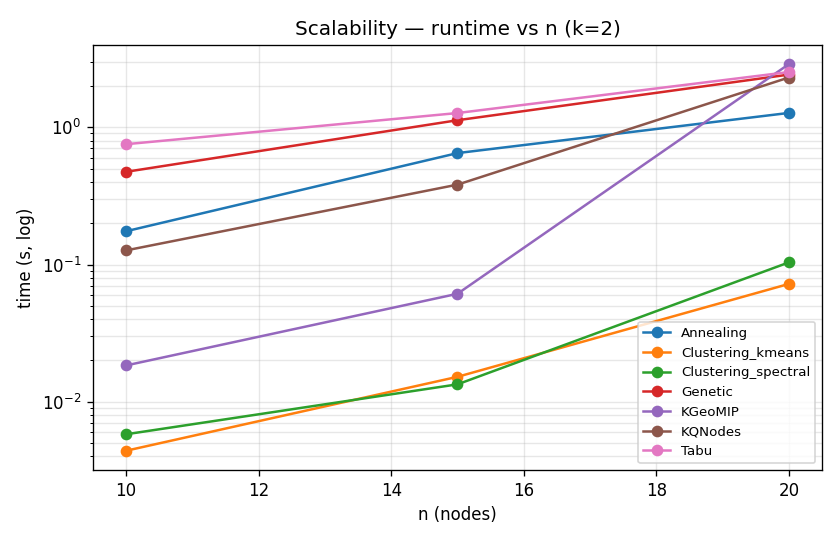
\includegraphics[width=0.48\textwidth]{scalability_k2.png}\hfill
	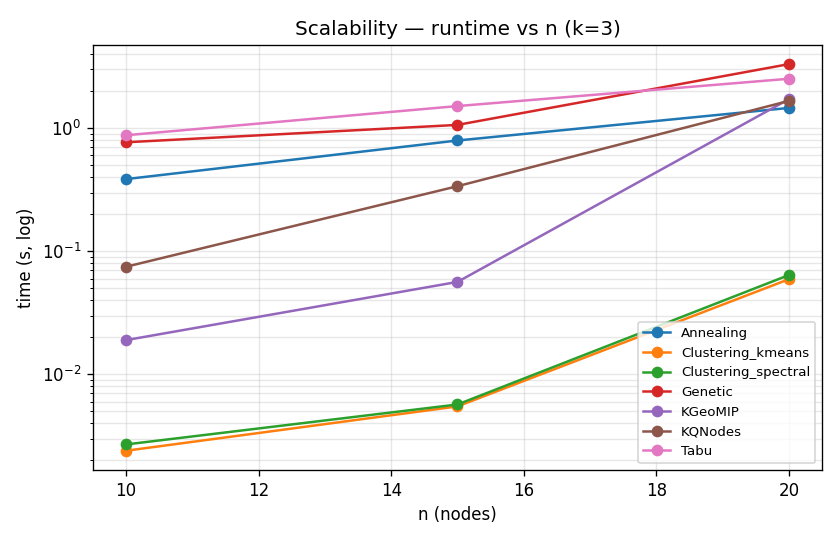
\includegraphics[width=0.48\textwidth]{scalability_k3.png}
	\caption{Escalabilidad (tiempo vs $n$, escala log) para $k=2$ (izq.) y $k=3$
		(der.) sobre el benchmark N10A/N15A/N20A. KGeoMIP es varias veces más rápido que
		KQNodes a $n$ pequeño ($\sim$5--7×) y ambas convergen hacia $n=20$; a $n\ge 22$ la
		relación se invierte (Tabla~\ref{tab:time}).}
	\label{fig:scal}
\end{figure}

\begin{figure}[H]
	\centering
	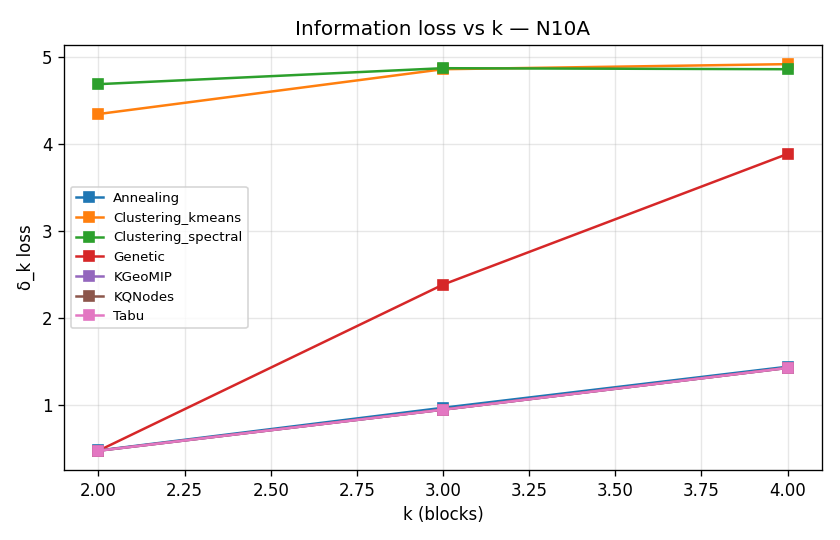
\includegraphics[width=0.48\textwidth]{loss_vs_k_N10A.png}\hfill
	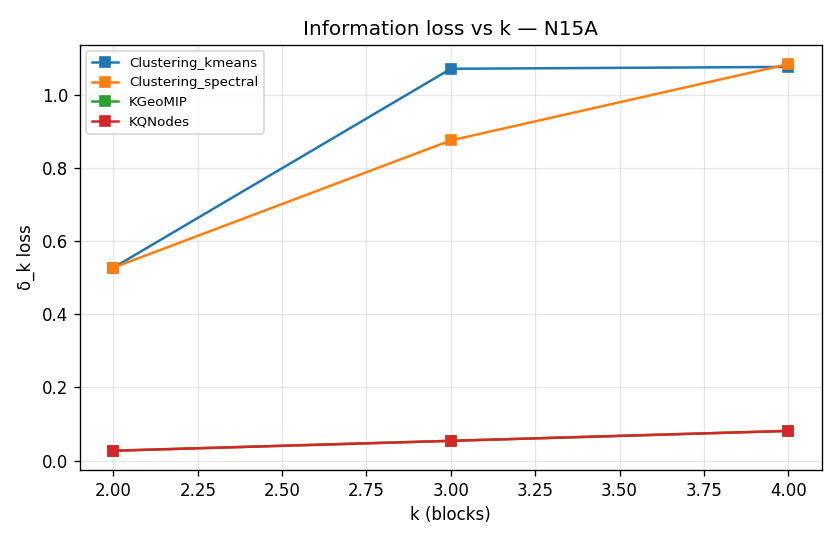
\includegraphics[width=0.48\textwidth]{loss_vs_k_N15A.png}
	\caption{Pérdida $\dk$ vs $k$ en N10A (izq.) y N15A (der.): monótona creciente,
		como exige la semántica estricta.}
	\label{fig:lossk}
\end{figure}

\begin{figure}[H]
	\centering
	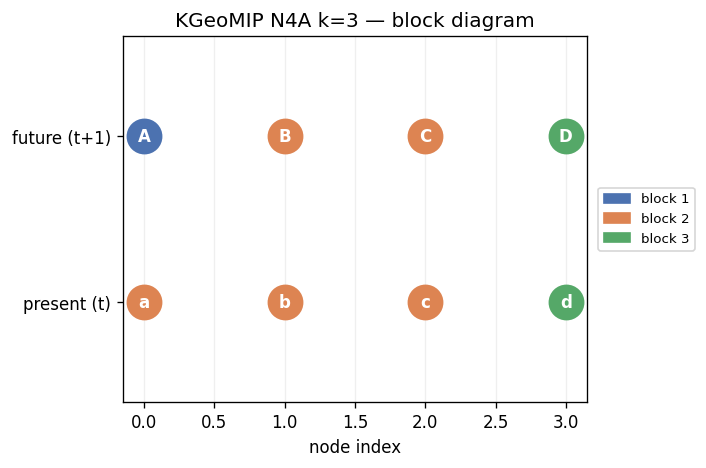
\includegraphics[width=0.46\textwidth]{partition_KGeoMIP_N4A_k3.png}\hfill
	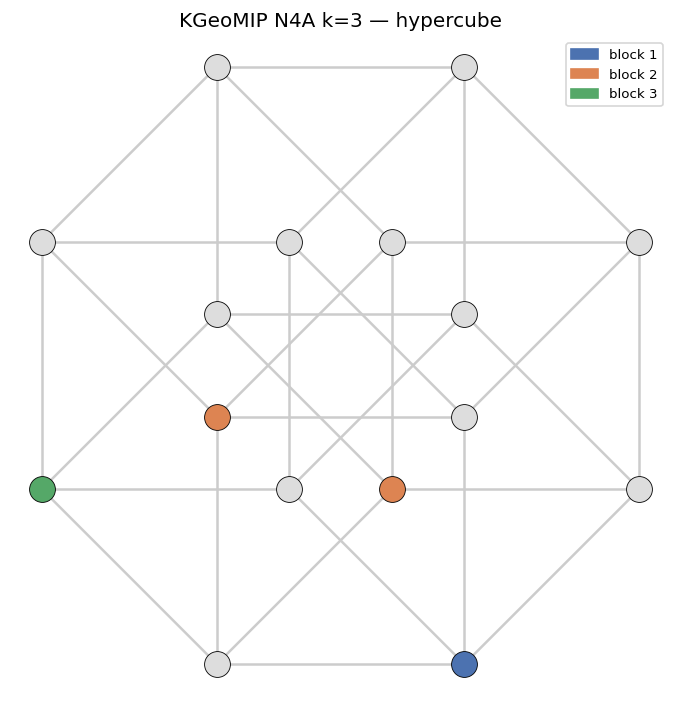
\includegraphics[width=0.46\textwidth]{hypercube_KGeoMIP_N4A_k3.png}
	\caption{$k$-partición hallada (N4A, $k=3$): diagrama de bloques presente/futuro
		(izq.) y proyección del hipercubo de nodos (der.).}
	\label{fig:viz}
\end{figure}

\subsection{Visualización interactiva e interfaz web}
Las mismas vistas se ofrecen de forma \textbf{interactiva} (Plotly) mediante
\texttt{src/viz/interactive.py}: diagrama de bloques de la partición con
\emph{hover} por bloque, $\dk$ vs $k$ y escalabilidad con ejes navegables.
\texttt{scripts/make\_interactive.py} las exporta como HTML autocontenido
(\texttt{plotly.js} por CDN). Todo se integra en una \textbf{interfaz web}
(Streamlit, \texttt{streamlit\_app.py}) que permite, sin línea de comandos:
generar una TPM desde el navegador, elegir estrategia/$k$/máscaras, y obtener la
partición, su $\dk$, la distribución marginal y las figuras estática e
interactiva. El registro sin interfaz (\emph{headless}) \texttt{src/funcs/runner.py}
(\texttt{run\_analysis}) es el núcleo compartido por la UI y los scripts.
La interfaz web vive en \texttt{streamlit\_app.py}.

\subsection{Análisis de resultados}
\begin{itemize}
	\item \textbf{KGeoMIP $\equiv$ KQNodes en calidad:} ambas hallan la misma
	      pérdida (diferencias $\le 10^{-4}$ por desempates), confirmando que comparten
	      el motor voraz y la métrica $\dk$.
	\item \textbf{Núcleo $\gg$ línea base:} las estrategias núcleo superan al
	      clustering por $\sim\!10\times$ en N10A y $\sim\!20\times$ en N15A; el clustering
	      optimiza una métrica de grafo, no $\dk$.
	\item \textbf{Costo relativo según la escala:} en redes pequeñas KQNodes es
	      $\sim\!7\times$ más lento que KGeoMIP por la búsqueda Queyranne, pero a $n=22$ y
	      $n=25$ la relación se invierte: KQNodes resuelve el subsistema completo en
	      $\approx 4$\,s y $\approx 25$\,s frente a $\approx 9$\,s y $\approx 100$\,s de
	      KGeoMIP (Tabla~\ref{tab:time}), porque su preparación es más barata que la tabla
	      de costos geométrica a esos tamaños.
	\item \textbf{Monotonía:} $\dk$ crece con $k$ (Fig.~\ref{fig:lossk}), coherente
	      con que más bloques destruyen más información.
	\item \textbf{Ambas escalan a $n=25$:} KGeoMIP y KQNodes llenan la tabla oficial
	      completa hasta N25A puntuando cada celda con $\dk$ (Tabla~\ref{tab:loss}). El
	      salto de tiempo de $n=20$ a $n=25$ valida empíricamente la cota $\bigO(2^n)$ de
	      la preparación; el límite práctico es la memoria, no el tiempo
	      (§\ref{sec:limites}).
	\item \textbf{Metaheurísticas (Tabla~\ref{tab:meta}):} la \emph{búsqueda tabú}
	      iguala la mejor pérdida convergente en toda la tabla; el \emph{recocido} se le aproxima salvo en
	      $k$ alto; la \emph{genética} acierta en $k=2$ pero se degrada al crecer $k$,
	      pues el espacio $k^{2n}$ excede el presupuesto de $\sim\!1200$ evaluaciones por
	      defecto. Es el comportamiento esperado de una metaheurística sin reinicio y
	      refuerza que las estrategias núcleo (deterministas) son la mejor opción aquí.
\end{itemize}

\subsection{Interpretación de los resultados}
\label{sec:interpretacion}
Más allá de los números, conviene leer qué significan para la teoría y para el uso
del sistema.

\paragraph{Qué dice la pérdida sobre el sistema.} Una pérdida $\dk$ baja indica que
el sistema se puede romper en $k$ bloques perdiendo poca información integrada: sus
partes son casi independientes en su efecto causal. Una pérdida alta indica lo
contrario, que el todo depende fuertemente de la interacción entre bloques. N15B es
el caso extremo: $\dk=0$ para todo $k$, así que esa red determinista es separable
sin pérdida. En las demás redes la pérdida crece de forma ordenada con $k$ (cada
bloque adicional rompe más estructura), lo que es la firma esperada de una semántica
estricta de partición.

\paragraph{Por qué las dos estrategias núcleo coinciden.} KGeoMIP parte de cortes
geométricos guiados por la tabla de costos y KQNodes de una secuencia submodular tipo
Queyranne, pero ambas refinan con la misma pérdida $\dk$ y, sobre el subsistema
completo de cada red, llegan al mismo valor. Que dos búsquedas con orígenes distintos
converjan al mismo mínimo es la evidencia práctica de optimalidad que se puede dar a
esta escala, donde enumerar todas las $k$-particiones es inviable. Las metaheurísticas
independientes (sobre todo Tabú) refuerzan esa coincidencia.

\paragraph{Cuándo usar cada una.} En redes pequeñas las dos son intercambiables y muy
rápidas. A $n=22$ y $n=25$ KQNodes resuelve el subsistema completo más rápido que
KGeoMIP (su preparación es más barata que la tabla de costos geométrica), así que es
la opción preferible cuando el tiempo importa. KGeoMIP sigue siendo útil porque su
\emph{cut pool} geométrico aporta diversidad de cortes (a veces halla una partición
distinta de igual $\dk$) y es más rápida en $n$ pequeño; en la franja verificable por
fuerza bruta ($n\le 6$) ambas tienen una tasa de acierto exacto equivalente. La
recomendación operativa es ejecutar ambas y tomar el mínimo.

\paragraph{Dónde está el límite.} El techo de $n\approx 25$ no es de tiempo sino de
memoria: la tabla de costos de KGeoMIP a subsistema completo de $n=25$ ronda los
$8{,}4$~GB. En una máquina de 16~GB eso obliga a ejecutar las filas grandes en serie,
que es lo que fija el tiempo total de llenar la tabla oficial. Subir de $25$ pediría
o más memoria o un esquema que evite materializar la tabla completa.

\subsection{Validación de correctitud}
La validación se ejecuta con \texttt{uv run scripts/validate.py}, que tiene tres
subcomandos: \texttt{correctness}, \texttt{optimality} y \texttt{external}.

\subsubsection{Frente al óptimo exacto y al legado $k=2$}
\begin{itemize}
	\item \textbf{Regresión $k=2$:} KGeoMIP y KQNodes reproducen exactamente GeoMIP
	      y QNodes legados.
	\item \textbf{Oráculo:} sobre los casos golden, el núcleo (BruteForce$\equiv$
	      GeoMIP) coincide $21/21$; en $k=2$ KGeoMIP iguala el óptimo exacto y KQNodes
	      acierta $9/10$. Para $k\ge 3$ ambas son voraces y pueden quedar por encima del
	      exacto (§\ref{sec:interpretacion}).
	\item \textbf{Consistencia:} \texttt{loss}\,$=\dk$ y \texttt{loss}\,$\ge$ óptimo
	      exacto en $18/18$ casos del verificador; \texttt{float32} igual a
	      \texttt{float64} dentro de $10^{-5}$.
\end{itemize}

\subsubsection{Frente al proyecto original de la docente}
La única referencia externa de la que se reporta es el proyecto original entregado
por la docente (\texttt{.core/core\_00}), cuyo repositorio es
\href{https://github.com/JuManoel/projecto-analisis-20261}{\texttt{github.com/JuManoel/projecto-analisis-20261}}.
El subcomando \texttt{external} comprueba dos cosas y mide los resultados:
\begin{itemize}
	\item \textbf{TPM idéntica:} el archivo \texttt{data/samples/N15A.csv} del que
	      muestreamos es idéntico byte a byte al que trae el proyecto original.
	\item \textbf{Reproducción de GeoMIP:} las filas de su
	      \texttt{resultados\_Geometric.xlsx} (N15A, TPM continua) se reproducen con nuestro
	      \texttt{GeometricSIA} dentro de la tolerancia \texttt{float32}. Tres filas medidas:
	      $0{,}0002500843$ vs $0{,}0002501011$; $0{,}0002678838$ vs $0{,}0002678633$
	      (dos veces). Las seis primeras filas reproducen con \texttt{OK}.
\end{itemize}

\subsubsection{Re-evaluación de las particiones almacenadas}
Cada celda de la tabla oficial guarda la partición, su pérdida y su tiempo. El
subcomando \texttt{external --verify-partitions} vuelve a leer cada partición, la
valida como $k$-partición estricta (cobertura y disjunción de la
sección~\ref{sec:def-kpart}) y la re-puntúa con la $\dk$ oficial sobre el
subsistema reconstruido. Sobre las cinco hojas de la tabla (N10A, N15B, N20A, N22A,
N25A), las $1992$ celdas llenas dan $0$ particiones inválidas y $0$ desajustes
de pérdida: las particiones reportadas son las que realmente se evaluaron, no solo
sus números.

% ====================== 8. LIMITACIONES ======================
\section{Limitaciones y trabajo futuro}
\label{sec:limites}

\subsection{Limitaciones conocidas}
\begin{itemize}
	\item \textbf{Techo de escala $n\approx 25$:} KGeoMIP y KQNodes llenan la tabla
	      oficial completa hasta N25A puntuando cada celda con $\dk$. El límite es la
	      memoria: la tabla de costos de KGeoMIP a subsistema completo de $n=25$ tiene un
	      pico de $\approx 8{,}4$~GB, así que en una máquina de 16~GB las filas grandes se
	      ejecutan en serie. No se promete escalar más allá de $n\approx 25$.
	\item \textbf{Tiempos a $n=25$:} sobre el subsistema completo de N25A (la fila más
	      cara), KGeoMIP resuelve $k=2..5$ en $\approx 101$~s y KQNodes en $\approx 26$~s.
	      El grueso es la preparación compartida (tabla de costos y \emph{cut pool}), que se
	      carga a $k=2$; los $k=3,4,5$ solo refinan y tardan décimas de segundo. Las filas
	      con subsistema más pequeño son mucho más baratas.
	\item \textbf{Optimalidad:} el motor voraz es heurístico; no garantiza la
	      $k$-MIP global (sí factibilidad, monotonía y validación contra el exacto en $n$
	      pequeño y convergencia de estrategias independientes a mayor escala).
\end{itemize}

\subsection{Supuestos y restricciones}
TPM determinista binaria; independencia condicional del repertorio de efecto (que
habilita la EMD-efecto analítica $\bigO(n)$); GIL activo en Python 3.14.5, por lo
que el paralelismo es por procesos, no por hilos.

\subsection{Mejoras potenciales y trabajo futuro}
La marginalización local, la carga en \texttt{uint8} y las metaheurísticas
comparativas ya están implementadas (secciones~\ref{sec:marginal-local}
y~\ref{sec:metaheur}). Lo que queda como trabajo futuro:
\begin{itemize}
	\item Llenado por lotes consciente de la memoria: paralelizar por procesos solo
	      las hojas que caben en RAM (hasta $n\approx 20$) y dejar las filas grandes en
	      serie, para recortar el tiempo de la tabla completa sin arriesgar OOM.
	\item Refinamiento con anticipación (\emph{look-ahead}) o búsqueda en haz
	      (\emph{beam search}) para acercarse al
	      óptimo global manteniendo costo polinómico.
	\item Aceleración GPU solo si el volumen justifica la transferencia H2D
	      (analizado: no rentable para los tamaños actuales).
\end{itemize}

% ====================== 9. APÉNDICES ======================
\section{Apéndices técnicos}

\subsection{Reducción $k=2 \Rightarrow$ bipartición legada}
\textbf{Proposición.} Para $k=2$, \textsc{GreedyKPartition} ejecuta exactamente un
refinamiento y el resultado coincide con la bipartición de la estrategia base.\\
\emph{Bosquejo.} El bucle \texttt{while} corre mientras $|\mathit{blocks}|<2$, es
decir una sola iteración partiendo de $[(F,M)]$. El único bloque es el universo
completo, de modo que dividirlo con un corte $c$ produce $(c,\bar c)$, que es la
bipartición candidata original. Como el pool y la métrica $\dk$ son los del método
base, se selecciona la misma bipartición. $\square$

\subsection{Reproducción de figuras y diagramas}
\begin{lstlisting}[style=sh,caption={Comandos de reproducción.}]
# Tabla y metricas
uv run scripts/run_benchmark.py
uv run scripts/validate.py correctness
# Figuras (matplotlib) y visualizacion de particiones
uv run scripts/make_figures.py
uv run scripts/make_viz.py --net N4A --k 3 --strategy KGeoMIP
# Diagramas UML editables (PlantUML)
plantuml docs/manuales/diagrams/*.puml
\end{lstlisting}

\subsection{Uso de inteligencia artificial generativa}
Durante el desarrollo se utilizó \textbf{Claude Code (Opus 4.8)} como asistente,
documentado entrada por entrada en \texttt{logs/ai\_agent\_changelog.md} (con el
\emph{prompt} del usuario, parámetros reales y decisiones).

\paragraph{Etapas y ejemplos.}
\begin{itemize}
	\item \textbf{Diseño:} extracción del motor voraz compartido
	      (\texttt{greedy\_k\_partition}) y decisión de semántica estricta tras medir que
	      la semántica débil degeneraba $k>2$ a bipartición.
	\item \textbf{Implementación:} vectorización de \texttt{CostTable}, conversión a
	      \texttt{float32}, infraestructura PCD (\texttt{parallel.py}) y visualización
	      (\texttt{src/viz}).
	\item \textbf{Depuración/optimización:} perfilado con \texttt{pyinstrument};
	      hallazgo de que Numba en lotes pequeños era $\sim\!70\%$ más lento (revertido) y
	      de que la marginalización domina el costo.
	\item \textbf{Documentación:} estructuración de manuales, diagramas y tablas.
\end{itemize}

\paragraph{Reflexión crítica.} La IA aceleró tareas mecánicas (vectorización, código
repetitivo, redacción) y propuso refactorizaciones útiles; sin embargo, varias
afirmaciones de evaluación automática se basaron en código obsoleto y debieron
\emph{verificarse} contra el repositorio real (regla ``verificar, no asumir''). El
criterio de validación contra oráculo y micro-mediciones (\emph{microbenchmarks})
aisladas fue imprescindible para no aceptar mejoras ilusorias. La comprensión profunda
del algoritmo y la responsabilidad de las decisiones permanecen en el equipo.

\subsection{Referencias}
\begin{thebibliography}{99}
	\bibitem{tononi} G. Tononi. \emph{An information integration theory of
		consciousness}. BMC Neuroscience, 5:42, 2004.
	\bibitem{oizumi} M. Oizumi, L. Albantakis, G. Tononi. \emph{From the phenomenology
		to the mechanisms of consciousness: Integrated Information Theory 3.0}. PLoS
	Computational Biology, 10(5):e1003588, 2014.
	\bibitem{pyphi} W. Mayner et al. \emph{PyPhi: A toolbox for integrated information
		theory}. PLoS Computational Biology, 14(7):e1006343, 2018.
	\bibitem{queyranne} M. Queyranne. \emph{Minimizing symmetric submodular
		functions}. Mathematical Programming, 82:3--12, 1998.
	\bibitem{nwf} G. Nemhauser, L. Wolsey, M. Fisher. \emph{An analysis of
		approximations for maximizing submodular set functions---I}. Mathematical
	Programming, 14:265--294, 1978.
	\bibitem{rubner} Y. Rubner, C. Tomasi, L. Guibas. \emph{The Earth Mover's Distance
		as a metric for image retrieval}. International Journal of Computer Vision,
	40(2):99--121, 2000.
	\bibitem{vonluxburg} U. von Luxburg. \emph{A tutorial on spectral clustering}.
	Statistics and Computing, 17(4):395--416, 2007.
	\bibitem{kirkpatrick} S. Kirkpatrick, C. Gelatt, M. Vecchi. \emph{Optimization by
		simulated annealing}. Science, 220(4598):671--680, 1983.
	\bibitem{glover} F. Glover. \emph{Future paths for integer programming and links to
		artificial intelligence}. Computers \& Operations Research, 13(5):533--549, 1986.
	\bibitem{holland} J. Holland. \emph{Adaptation in Natural and Artificial Systems}.
	University of Michigan Press, 1975.
	\bibitem{docproj} Universidad de Caldas. \emph{Proyecto K-QGMIP — Especificación}
	(\texttt{docs/Proyecto\_KQMIP.md}), 2026-1.
\end{thebibliography}

\end{document}
